\documentclass[12pt,a4paper]{article}

\usepackage{fontspec}
\usepackage{polyglossia}
\setmainlanguage[babelshorthands=true]{russian}
\setotherlanguage{english}

\setmainfont{Times New Roman}
\newfontfamily{\cyrillicfont}{Times New Roman}
\setsansfont{Arial}
\setmonofont{Courier New}
\newfontfamily{\cyrillicfonttt}{Courier New}

\usepackage{graphicx}
\usepackage{xcolor}
\usepackage{hyperref}
\usepackage{longtable}
\usepackage{booktabs}
\usepackage{array}
\usepackage{titlesec}
\usepackage{fancyhdr}
\usepackage{geometry}
\usepackage{caption}
\usepackage{enumitem}
\usepackage{amsmath}

\geometry{left=2.5cm,right=2cm,top=2cm,bottom=2cm}

\hypersetup{
    colorlinks=true,
    linkcolor=blue,
    urlcolor=blue,
    citecolor=blue
}

\pagestyle{fancy}
\fancyhf{}
\fancyhead[L]{\leftmark}
\fancyhead[R]{\thepage}
\renewcommand{\headrulewidth}{0.4pt}

\titleformat{\section}{\Large\bfseries}{\thesection}{1em}{}
\titleformat{\subsection}{\large\bfseries}{\thesubsection}{1em}{}
\titleformat{\subsubsection}{\normalsize\bfseries}{\thesubsubsection}{1em}{}

\renewcommand{\arraystretch}{1.2}

\newcommand{\linktarget}[1]{\hypertarget{#1}{}}
\newcommand{\linkref}[1]{\hyperlink{#1}{#1}}

% Simplify wiki links in text
\newcommand{\wikilink}[1]{#1}

\begin{document}

% ─── Title Page ──────────────────────────────────────────────────────────────
\begin{titlepage}
\centering
\vspace*{4cm}

{\Huge\bfseries BulbaInvest\\[0.5cm]
\large Учебная брокерская платформа}

\vspace{1.5cm}

{\Large Техническая документация и база знаний}

\vspace{1cm}

{\large Версия 1.0\\[0.3cm]
\today}

\vfill

{\itshape Имитация брокерской экосистемы для учебных целей}
\end{titlepage}

% ─── Table of Contents ──────────────────────────────────────────────────────
\tableofcontents
\newpage

% ═════════════════════════════════════════════════════════════════════════════
% PART 1: TECHNICAL SPECIFICATION
% ═════════════════════════════════════════════════════════════════════════════
\part{Техническое задание}

\section{Назначение системы}

Система предназначена для учебной имитации брокерской платформы, в которой
пользователь может авторизоваться, просматривать рынок акций, получать котировки,
анализировать графики, пополнять учебный кошелёк, покупать и продавать активы,
создавать заявки и просматривать портфель.

Продукт состоит из Android-приложения и backend-сервисов, которые совместно
моделируют работу инвестиционного приложения и брокерской инфраструктуры без
подключения к реальной бирже и без реальных денежных операций.

\section{Цели разработки}

Цель разработки --- создать готовый MVP учебного стартап-продукта для демонстрации
полного цикла работы брокерской платформы:

\begin{itemize}
    \item мобильное приложение для клиента-инвестора;
    \item backend API для авторизации, профиля, кошельков, портфеля и сделок;
    \item сервис генерации и выдачи котировок;
    \item сервис хранения истории котировок и построения свечных графиков;
    \item механизм покупки и продажи акций;
    \item механизм P2P-заявок между пользователями;
    \item запуск системы в контейнеризированном окружении;
    \item проверка работы системы под учебной нагрузкой до 10\,000 клиентов.
\end{itemize}

\section{Пользователи системы}

\begin{longtable}{p{4cm}p{10cm}}
\toprule
\textbf{Роль} & \textbf{Описание} \\
\midrule
\endhead
Клиент / инвестор &
Основной пользователь Android-приложения. Авторизуется по email-коду,
просматривает рынок, пополняет баланс, покупает и продаёт акции, управляет
портфелем и заявками. \\
Мобильное приложение &
Android-клиент, который взаимодействует с backend через HTTP API и WebSocket. \\
Backend-сервисы &
Внутренние сервисы системы, обеспечивающие доменную логику, котировки, историю
графиков и проксирование клиентских запросов. \\
Сервис рынка &
Внутренний сервис, который имитирует биржу, обновляет котировки и хранит
доступное количество акций компании. \\
\bottomrule
\end{longtable}

\section{Функциональные требования}

{\small
\begin{longtable}{p{1.2cm}p{3cm}p{9.5cm}}
\toprule
\textbf{ID} & \textbf{Требование} & \textbf{Описание} \\
\midrule
\endhead
FR-01  & Android-приложение        & Пользователь работает с системой через мобильное Android-приложение. \\
FR-02  & Авторизация по email-коду & Пользователь запрашивает код на email, подтверждает его и получает JWT-токен. \\
FR-03  & Хранение токена на клиенте & Android-приложение сохраняет JWT и использует его для авторизованных запросов. \\
FR-04  & Просмотр профиля          & Пользователь может получить данные текущего аккаунта. \\
FR-05  & Обновление профиля        & Пользователь может изменить имя профиля. \\
FR-06  & Просмотр кошельков        & Пользователь видит свои учебные кошельки и доступный баланс. \\
FR-07  & Пополнение учебного баланса & Пользователь может пополнить учебный кошелёк для выполнения операций покупки. \\
FR-08  & Управление кошельками     & Система предусматривает создание кошелька, выбор кошелька по умолчанию и удаление кошелька. \\
FR-09  & Просмотр портфеля         & Пользователь видит список купленных активов, количество акций и среднюю цену покупки. \\
FR-10  & Просмотр позиции по тикеру & Пользователь может получить информацию по отдельной позиции портфеля. \\
FR-11  & Просмотр рынка            & Пользователь видит список доступных тикеров и актуальные цены. \\
FR-12  & Получение текущих котировок & Система выдаёт актуальные котировки акций через REST API и WebSocket. \\
FR-13  & Автоматическое обновление котировок & Сервис рынка периодически обновляет цены и публикует обновления для клиентов и сервисов. \\
FR-14  & Просмотр информации об активе & Пользователь может открыть экран конкретной акции и увидеть текущую цену и детали инструмента. \\
FR-15  & Просмотр графика цены     & Пользователь может просматривать свечной график цены по выбранному тикеру. \\
FR-16  & История котировок         & Система сохраняет историю котировок и отдаёт агрегированные OHLCV-свечи. \\
FR-17  & Покупка акций у компании  & Пользователь может купить акции у имитируемой компании/рынка при наличии средств и доступного inventory. \\
FR-18  & Продажа акций компании    & Пользователь может продать акции обратно компании при наличии позиции в портфеле. \\
FR-19  & Создание заявки на продажу & Пользователь может выставить sell order на продажу своих акций. \\
FR-20  & Просмотр стакана заявок   & Пользователь может просматривать активные заявки на продажу по тикеру. \\
FR-21  & Покупка из стакана        & Пользователь может купить акции из order book по заданной цене. \\
FR-22  & Покупка конкретной заявки  & Пользователь может купить выбранную заявку другого пользователя. \\
FR-23  & Отмена заявки             & Пользователь может отменить свою активную заявку на продажу. \\
FR-24  & История сделок            & Пользователь может получить историю своих операций покупки и продажи. \\
FR-25  & Хранение пользовательских данных & Система хранит пользователей, кошельки, портфели, заявки и сделки в БД. \\
FR-26  & Хранение текущих котировок & Система хранит актуальные котировки в Redis для быстрого чтения. \\
FR-27  & Хранение истории котировок & Система хранит исторические котировки в ClickHouse. \\
FR-28  & WebSocket-обновления       & Android-приложение получает live-обновления котировок через WebSocket. \\
FR-29  & API Gateway               & Клиент обращается к единой входной точке, которая маршрутизирует запросы к backend-сервисам. \\
FR-30  & Обработка ошибок           & API возвращает структурированные ошибки, а клиент отображает сообщения пользователю. \\
FR-31  & Межсервисная интеграция    & Сервисы обмениваются данными через HTTP, Redis Pub/Sub, Redis Streams и общую Docker-сеть. \\
FR-32  & Защита от повторной обработки & Операции изменения inventory используют idempotency key. \\
FR-33  & Логирование                & Сервисы ведут логи запросов, ошибок и фоновых операций. \\
FR-34  & Запуск через Docker Compose & Backend и инфраструктура запускаются через Docker Compose. \\
FR-35  & Нагрузочное тестирование   & Система проверена учебной имитацией нагрузки до 10\,000 клиентов. \\
\bottomrule
\end{longtable}
}

\section{Нефункциональные требования}

\subsection{Производительность}

Система должна поддерживать учебную нагрузку до 10\,000 клиентов. Для снижения
нагрузки на backend live-котировки передаются через WebSocket, а история котировок
записывается в ClickHouse батчами. Текущие котировки должны читаться быстро за
счёт хранения последних значений в Redis.

\subsection{Надёжность}

Система должна проверять баланс пользователя, доступное количество акций, статус
заявки и корректность входных данных перед выполнением сделки.

Операции с кошельками, портфелем, ордерами и сделками должны сохраняться атомарно
в пределах доменной БД. Операции изменения inventory должны быть идемпотентными.

\subsection{Безопасность}

Пользовательские endpoints должны требовать JWT-авторизацию. JWT выдаётся только
после подтверждения email-кода. Секреты, пароли и адреса сервисов должны
передаваться через переменные окружения.

\subsection{Масштабируемость}

Система должна быть разделена на компоненты по ответственности: мобильный клиент,
Gateway, доменная логика, сервис рынка, сервис графиков и инфраструктурные
хранилища. Котировки должны распространяться через Redis Pub/Sub, чтобы несколько
потребителей могли получать обновления независимо.

\subsection{Сопровождаемость}

Код должен быть разделён на слои: UI, repository, network client, routes, services,
database, external integrations. API-контракты должны быть описаны в документации и
соответствовать реализации. Миграции и схемы хранения должны храниться в
репозитории.

\subsection{Логирование и мониторинг}

Все backend-сервисы должны иметь health endpoints. Система должна логировать
HTTP-запросы, ошибки интеграции, ошибки обработки сообщений и фоновые операции.

\subsection{Хранение данных}

Пользовательские данные, кошельки, портфели, ордера и сделки хранятся в PostgreSQL.
Текущие котировки и служебные временные данные хранятся в Redis. История котировок
хранится в ClickHouse.

\subsection{Развёртывание}

Backend-сервисы и инфраструктура должны запускаться через Docker Compose.
Android-приложение должно собираться как отдельный Gradle-проект. Конфигурация
окружения должна задаваться через .env и application config.

\subsection{API и обработка ошибок}

API должно использовать JSON. Ошибки валидации должны возвращать понятное
сообщение. Ошибки отсутствующих данных должны возвращать 404. Ошибки конфликтов
бизнес-логики должны возвращать 409. Gateway должен корректно обрабатывать
недоступность downstream-сервисов.

\section{Требования к данным}

\begin{longtable}{p{3cm}p{5cm}p{7cm}}
\toprule
\textbf{Данные} & \textbf{Сущность / хранилище} & \textbf{Назначение} \\
\midrule
\endhead
Пользователь & \texttt{users} & Хранение профиля клиента: id, email, имя, даты создания и обновления. \\
Кошелёк & \texttt{user\_wallets} & Хранение учебного баланса, валюты, зарезервированной суммы и признака кошелька по умолчанию. \\
Портфель & \texttt{portfolio\_positions} & Хранение позиций пользователя по тикерам, количества, зарезервированного количества и средней цены покупки. \\
Заявка & \texttt{sell\_orders} & Хранение P2P-заявок на продажу акций, цены, количества и статуса. \\
Сделка & \texttt{trades} & Хранение истории исполненных операций: покупатель, продавец, тикер, количество, цена, сумма и тип сделки. \\
Текущая котировка & Redis \texttt{market:stocks} & Быстрое получение актуальной цены и доступного количества акций. \\
Событие котировки & Redis channel \texttt{market.quotes.updated} & Рассылка обновлений котировок между сервисами и клиентскими подписками. \\
История котировок & ClickHouse \texttt{quotes} & Хранение time-series данных для построения свечей и графиков. \\
Inventory компании & \texttt{market\_company\_inventory} & Хранение доступного количества акций у компании/рынка. \\
Код авторизации & Redis с TTL & Временное хранение email-кодов входа. \\
Idempotency result & Redis & Хранение результата операции inventory для защиты от повторной обработки. \\
\bottomrule
\end{longtable}

\section{Требования к API}

\subsection{Gateway и клиентский доступ}

\begin{longtable}{p{1.5cm}p{4cm}p{4cm}p{5cm}}
\toprule
\textbf{Метод} & \textbf{Путь} & \textbf{Назначение} & \textbf{Входные / Выходные данные} \\
\midrule
\endhead
GET & \texttt{/health} & Проверка состояния Gateway & --- / \texttt{\{status: ok\}} \\
Any & \texttt{/api/**} & Проксирование клиентских запросов к backend & Method, path, query, headers, body / Ответ backend \\
GET & \texttt{/api/tickers} & Получение списка тикеров & JWT / Список тикеров \\
GET & \texttt{/api/quotes/\{ticker\}/latest} & Последняя котировка & JWT, ticker / Котировка \\
GET & \texttt{/api/quotes/\{ticker\}/stats} & Получение свечей & JWT, ticker, granularity / OHLCV-свечи \\
WS & \texttt{/ws/quotes} & Live-подписка на котировки & tickers / JSON-массив котировок \\
\bottomrule
\end{longtable}

\subsection{Пользователь и авторизация}

\begin{longtable}{p{1.5cm}p{4cm}p{4cm}p{5cm}}
\toprule
\textbf{Метод} & \textbf{Путь} & \textbf{Назначение} & \textbf{Входные / Выходные данные} \\
\midrule
\endhead
POST & \texttt{/api/auth/code/request} & Запрос кода авторизации & email / Статус отправки \\
POST & \texttt{/api/auth/code/confirm} & Подтверждение кода & email, code / JWT token \\
GET & \texttt{/api/users/me} & Получение пользователя & JWT / User \\
PATCH & \texttt{/api/users/me} & Изменение имени & JWT, name / User \\
\bottomrule
\end{longtable}

\subsection{Кошельки и портфель}

\begin{longtable}{p{1.5cm}p{4.5cm}p{3.5cm}p{5cm}}
\toprule
\textbf{Метод} & \textbf{Путь} & \textbf{Назначение} & \textbf{Входные / Выходные} \\
\midrule
\endhead
GET & \texttt{/api/wallets/me} & Список кошельков & JWT / Список Wallet \\
POST & \texttt{/api/wallets} & Создание кошелька & JWT, currency / Wallet \\
POST & \texttt{/api/wallets/\{id\}/make-default} & Выбор кошелька по умолчанию & JWT, walletId / Wallet \\
DELETE & \texttt{/api/wallets/\{id\}} & Удаление кошелька & JWT, walletId / Статус \\
POST & \texttt{/api/wallets/me/deposit} & Пополнение баланса & JWT, amount / Wallet \\
GET & \texttt{/api/portfolio} & Портфель пользователя & JWT / Список позиций \\
GET & \texttt{/api/portfolio/\{ticker\}} & Позиция по тикеру & JWT, ticker / Позиция \\
\bottomrule
\end{longtable}

\subsection{Сделки и заявки}

\begin{longtable}{p{1.5cm}p{5cm}p{3cm}p{5cm}}
\toprule
\textbf{Метод} & \textbf{Путь} & \textbf{Назначение} & \textbf{Входные / Выходные} \\
\midrule
\endhead
POST & \texttt{/api/trades/company/buy} & Покупка у компании & ticker, quantity, walletId / Trade \\
POST & \texttt{/api/trades/company/sell} & Продажа компании & ticker, quantity, walletId / Trade \\
GET & \texttt{/api/trades} & История сделок & JWT / Список Trade \\
GET & \texttt{/api/order-book/\{ticker\}} & Стакан заявок & JWT, ticker / OrderBook \\
POST & \texttt{/api/orders/sell} & Создание заявки на продажу & ticker, quantity, price / SellOrder \\
POST & \texttt{/api/orders/buy} & Покупка из стакана & ticker, quantity, maxPrice, walletId / Статус \\
POST & \texttt{/api/orders/sell/\{id\}/buy} & Покупка конкретной заявки & JWT, orderId / Статус \\
POST & \texttt{/api/orders/sell/\{id\}/cancel} & Отмена заявки & JWT, orderId / Статус \\
GET & \texttt{/api/orders/my} & Мои заявки & JWT / Список SellOrder \\
\bottomrule
\end{longtable}

\subsection{Сервис рынка и графиков}

\begin{longtable}{p{1.5cm}p{5cm}p{3cm}p{5cm}}
\toprule
\textbf{Метод} & \textbf{Путь} & \textbf{Назначение} & \textbf{Входные / Выходные} \\
\midrule
\endhead
GET & \texttt{/stocks} & Текущие котировки & --- / Список котировок \\
GET & \texttt{/stocks/\{ticker\}} & Котировка по тикеру & ticker / Котировка \\
POST & \texttt{/api/v1/inventory/decrement} & Уменьшение inventory & ticker, quantity, idempotencyKey / Результат \\
POST & \texttt{/api/v1/inventory/increment} & Увеличение inventory & ticker, quantity, idempotencyKey / Результат \\
GET & \texttt{/api/tickers} & Тикеры с историей & --- / Список тикеров \\
GET & \texttt{/api/quotes/\{ticker\}/latest} & Последняя цена & ticker / Quote \\
GET & \texttt{/api/quotes/\{ticker\}/stats} & OHLCV-свечи & ticker, granularity / Candles \\
\bottomrule
\end{longtable}

\section{Ограничения и допущения}

\begin{itemize}
    \item Система является учебной имитацией брокерской платформы.
    \item Все денежные операции выполняются в учебной валюте и не связаны с реальными платежами.
    \item Котировки генерируются сервисом имитации рынка.
    \item Список активов ограничен набором тикеров, поддерживаемых сервисом рынка.
    \item Нагрузка до 10\,000 клиентов рассматривается как учебная проверка масштабируемости MVP.
    \item Бизнес-логика упрощена по сравнению с реальной брокерской системой.
    \item Реальные юридические, биржевые и платёжные интеграции не входят в состав MVP.
\end{itemize}

\section{Критерии готовности}

MVP считается готовым, если:

\begin{itemize}
    \item Android-приложение собирается и запускается;
    \item пользователь может пройти авторизацию по email-коду;
    \item приложение сохраняет JWT и выполняет авторизованные запросы;
    \item backend запускается через Docker Compose;
    \item все основные сервисы имеют рабочий health endpoint;
    \item пользователь видит кошелёк и портфель;
    \item пользователь может пополнить учебный баланс;
    \item пользователь видит список тикеров и актуальные котировки;
    \item WebSocket передаёт обновления котировок;
    \item пользователь может открыть экран акции и посмотреть график;
    \item пользователь может купить и продать акции у компании;
    \item пользователь может создать, просмотреть, купить и отменить P2P-заявку;
    \item история сделок сохраняется и доступна через API;
    \item данные сохраняются в PostgreSQL, Redis и ClickHouse;
    \item нагрузочное тестирование или имитация клиентских запросов до 10\,000 клиентов выполнены;
    \item документация содержит техническое задание, OpenAPI-контракт и инструкции запуска.
\end{itemize}

% ═════════════════════════════════════════════════════════════════════════════
% PART 2: KNOWLEDGE BASE
% ═════════════════════════════════════════════════════════════════════════════
\newpage
\part{База знаний}

% ─── Architecture and Boundaries ─────────────────────────────────────────────
\section{Архитектура и границы сервисов}

Архитектура backend-системы описывает не только список сервисов, но и границы
ответственности между ними. Хорошая архитектура отвечает на вопросы: кто владеет
данными, кто принимает решения, как сервисы общаются, что происходит при ошибке
и где проходит внешний API.

\subsection{Microservices}

Microservice --- это самостоятельный сервис с понятной ответственностью,
собственным lifecycle, конфигурацией, контрактами и часто собственной базой
данных. Его размер менее важен, чем ясность границ.

Плохой microservice --- это просто часть монолита, вынесенная в отдельный процесс,
но продолжающая делить таблицы, бизнес-логику и внутренние модели с другими
частями системы. Хороший microservice владеет своим состоянием и предоставляет
наружу явный contract.

В trading-системах естественно выделяются разные зоны ответственности:
\begin{itemize}
    \item пользовательская доменная модель: users, wallets, portfolios, orders, trades;
    \item рыночная модель: quotes, available inventory, volatility, ticks;
    \item аналитическая модель: historical quotes, candles, aggregates;
    \item edge layer: внешний API, WebSocket, auth boundary, routing.
\end{itemize}

\subsection{Bounded context}

Bounded context --- это граница, внутри которой термины имеют устойчивый смысл.
Например, \texttt{price} в market context может быть текущей simulated quote, а
\texttt{price} в trade history --- уже зафиксированной ценой исполненной сделки.
Это разные факты, хотя название одинаковое.

Главное правило bounded context: у каждого факта должен быть один владелец. Если
два сервиса считают себя владельцами одного значения, возникает shared ownership.
Это почти всегда приводит к расхождениям.

\subsection{API Gateway}

API Gateway --- единая входная точка для клиентов. Он скрывает внутреннюю
топологию сервисов, маршрутизирует запросы, может проверять auth, добавлять
request id, логировать edge-запросы, применять rate limiting и держать WebSocket
endpoint.

Gateway полезен, когда клиенту не нужно знать адрес каждого сервиса. Клиент
обращается к одному public API, а gateway проксирует запросы во внутреннюю сеть.

Но gateway не должен становиться вторым domain service. Его задача --- edge-логика,
а не правила сделок. Если gateway начинает решать, можно ли пользователю купить
акцию, это признак утечки business logic.

\subsection{Service contracts}

Contract --- это обещание сервиса. Он описывает endpoints, payloads, status codes,
message schemas, retry behavior и idempotency rules.

Контракты бывают:
\begin{itemize}
    \item HTTP contracts: REST endpoints, OpenAPI, status codes;
    \item message contracts: JSON payloads в broker или stream;
    \item WebSocket contracts: формат сообщений и правила подписки;
    \item operational contracts: health checks, readiness, timeouts.
\end{itemize}

В distributed system нельзя полагаться на <<мы знаем, как оно внутри устроено>>.
Внутреннее устройство сервиса может меняться, но контракт должен оставаться
стабильным или версионироваться.

\subsection{Event-driven architecture}

Event-driven architecture строится вокруг событий. Producer публикует факт,
consumer реагирует. Например, market service публикует \texttt{quotes updated},
gateway отправляет обновление клиентам, graph service сохраняет историю.

Важно различать events и commands:
\begin{itemize}
    \item \textbf{Event} сообщает, что что-то уже произошло: цена обновилась,
          order matched, user created. Event может читать много consumers.
    \item \textbf{Command} просит выполнить действие: уменьшить inventory, создать
          order, списать деньги. Command требует результата, обработки ошибок и
          часто idempotency.
\end{itemize}

Для live data подходят Pub/Sub-механизмы. Для критичных операций лучше использовать
durable streams, message queues или HTTP-команды с idempotency key.

\subsection{Практические правила}

\begin{itemize}
    \item Сначала определяют owners данных, потом выбирают протоколы взаимодействия.
    \item Сервис не должен напрямую писать в базу другого сервиса.
    \item Gateway не должен содержать core business logic.
    \item Contracts нужно документировать отдельно от внутренней реализации.
    \item Events подходят для распространения фактов, commands --- для действий с результатом.
    \item Если операция затрагивает несколько сервисов, нужно заранее продумать
          idempotency, retries и compensation.
\end{itemize}

% ─── Trading Domain ──────────────────────────────────────────────────────────
\newpage
\section{Trading domain}

Trading domain описывает пользователей, деньги, портфели, заявки, сделки и
рыночные операции. Даже в учебной системе эти понятия нужно моделировать
аккуратно, потому что ошибки быстро приводят к отрицательным балансам, двойной
продаже или расхождению истории.

\subsection{Основные сущности}

\begin{itemize}
    \item \textbf{User} --- участник системы.
    \item \textbf{Wallet} --- денежный счет пользователя. Содержит currency,
          amount и reserved amount.
    \item \textbf{Portfolio position} --- количество бумаг по конкретному ticker.
    \item \textbf{Order} --- заявка на покупку или продажу.
    \item \textbf{Trade} --- исполненная сделка.
    \item \textbf{Quote} --- текущая рыночная цена или snapshot рынка.
    \item \textbf{Inventory} --- количество бумаг, доступных у компании или
          market maker.
\end{itemize}

\subsection{Company trades и user trades}

Сделки можно разделить на два типа:
\begin{itemize}
    \item \textbf{Company trade} --- пользователь покупает у компании или продаёт
          компании. Здесь участвует внешний market context: нужно проверить или
          изменить inventory.
    \item \textbf{User trade} --- пользователь покупает у другого пользователя.
          В упрощённой системе это можно выполнить целиком внутри domain database.
\end{itemize}

Разница важна для consistency. User trade может быть атомарной SQL transaction.
Company trade часто становится distributed workflow, потому что затрагивает
несколько сервисов.

\subsection{Order book}

Order book --- список заявок. В полной биржевой системе есть buy side и sell side.
В упрощённой модели может быть только sell side: пользователи выставляют sell
orders, а покупатели выбирают конкретный order или покупают из стакана по
максимальной цене.

Order status обычно включает:
\begin{itemize}
    \item OPEN;
    \item PARTIALLY\_FILLED;
    \item MATCHED или FILLED;
    \item CANCELLED;
    \item EXPIRED.
\end{itemize}

\subsection{Matching}

Matching --- процесс подбора встречных заявок. Простая стратегия --- price-time
priority: сначала лучшая цена; при одинаковой цене --- более ранняя заявка.

Для покупки из sell book выбираются самые дешёвые open sell orders, пока не будет
набрано нужное quantity или пока цена не превысит max price.

\subsection{Reservation}

Reservation защищает от двойного расходования.

Если пользователь выставляет sell order, система резервирует quantity в portfolio.
Эти бумаги нельзя продать повторно до отмены или исполнения order.

Если пользователь создаёт buy order, можно резервировать деньги в wallet. Это
предотвращает ситуацию, где пользователь создал несколько заявок на одну и ту же
сумму.

\subsection{Trade consistency}

Сделка должна сохранять инварианты:
\begin{itemize}
    \item balance не уходит ниже нуля;
    \item reserved amount не превышает amount;
    \item reserved quantity не превышает quantity;
    \item trade history соответствует изменениям wallet и portfolio;
    \item order status соответствует фактическому исполнению.
\end{itemize}

Для локальных операций помогает SQL transaction. Для distributed операций нужны
idempotency, retries, compensation и reconciliation.

\subsection{Average buy price}

\texttt{average\_buy\_price} показывает среднюю цену покупки позиции. При докупке
бумаг пересчитывается weighted average:

\[
\text{newAverage} = \frac{\text{oldQty} \times \text{oldAvg} + \text{buyQty} \times \text{buyPrice}}{\text{oldQty} + \text{buyQty}}
\]

При продаже средняя цена обычно не меняется, уменьшается только quantity.

\subsection{Практические правила}

\begin{itemize}
    \item Деньги считать только decimal types.
    \item Все изменения wallet, portfolio, order и trade history выполнять
          атомарно, если они находятся в одной базе.
    \item Не позволять пользователю купить собственный order.
    \item Не исполнять closed order.
    \item При distributed trade использовать idempotency key.
    \item Отдельно хранить текущее состояние и историю событий.
\end{itemize}

% ─── Data Storage and Modeling ───────────────────────────────────────────────
\newpage
\section{Хранение данных и моделирование}

Data storage выбирают под workload. В backend-системе с trading domain обычно
нужны разные типы хранения: relational database для транзакций, Redis для быстрых
значений и сообщений, column-oriented database для аналитики.

\subsection{PostgreSQL как source of truth}

PostgreSQL хорошо подходит для доменной модели, где важны транзакции, constraints
и consistency. Пользователи, кошельки, портфели, ордера и сделки требуют
атомарных изменений.

Пример: при покупке order нужно:
\begin{enumerate}
    \item списать деньги покупателя;
    \item начислить деньги продавцу;
    \item изменить портфель продавца;
    \item изменить портфель покупателя;
    \item обновить status order;
    \item записать trade history.
\end{enumerate}

Все эти шаги должны быть выполнены в одной transaction. Если один шаг падает,
остальные должны откатиться.

\subsection{Flyway и миграции}

Миграции делают схему базы частью кода. Flyway применяет SQL-файлы в заданном
порядке и хранит историю применённых миграций.

Преимущества миграций:
\begin{itemize}
    \item схема воспроизводится в новом окружении;
    \item изменения БД проходят code review;
    \item можно понять, какая версия схемы нужна приложению;
    \item проще запускать локальные и тестовые окружения.
\end{itemize}

\subsection{Exposed и SQL abstraction}

Exposed --- Kotlin SQL library. Она позволяет описывать таблицы и писать
типизированные queries. Важно помнить, что ORM/DSL не отменяет понимания SQL.

Даже при использовании Exposed нужно понимать:
\begin{itemize}
    \item где открывается transaction;
    \item какие queries выполняются;
    \item какие indexes нужны;
    \item как работает isolation;
    \item где может возникнуть race condition.
\end{itemize}

\subsection{Wallet model}

Wallet хранит деньги пользователя. Минимальная модель:
\begin{itemize}
    \item \texttt{id};
    \item \texttt{user\_id};
    \item \texttt{currency};
    \item \texttt{amount};
    \item \texttt{reserved\_amount};
    \item \texttt{is\_default};
    \item timestamps.
\end{itemize}

\texttt{reserved\_amount} нужен для операций, где деньги блокируются заранее.
Например, если buy order создаётся до исполнения, сумму можно зарезервировать,
чтобы пользователь не потратил её дважды.

\subsection{Portfolio model}

Portfolio position хранит количество бумаг по ticker:
\begin{itemize}
    \item \texttt{user\_id};
    \item \texttt{ticker};
    \item \texttt{quantity};
    \item \texttt{reserved\_quantity};
    \item \texttt{average\_buy\_price}.
\end{itemize}

\texttt{reserved\_quantity} нужна для sell orders. Если пользователь выставил
акции на продажу, он не должен продать эти же акции повторно до отмены или
исполнения order.

\subsection{Trade history}

Trade history --- журнал исполненных сделок. Он не заменяет текущее состояние
wallet или portfolio, но нужен для истории пользователя, аудита, аналитики и
сверок.

Trade обычно содержит:
\begin{itemize}
    \item buyer;
    \item seller;
    \item ticker;
    \item quantity;
    \item execution price;
    \item total amount;
    \item trade type;
    \item created time.
\end{itemize}

\subsection{Деньги и Decimal}

Деньги нельзя считать через floating point. Для финансовой логики нужны decimal
types: \texttt{BigDecimal} в приложении и \texttt{NUMERIC} или \texttt{DECIMAL}
в базе.

Floating point допустим для симуляции графиков или неофициальных вычислений, но
не для source of truth по балансу.

Практическое правило: все значения, которые влияют на wallet, portfolio и
settlement, должны проходить через decimal.

\subsection{Indexes и constraints}

Constraints защищают данные:
\begin{itemize}
    \item unique email;
    \item unique \texttt{(user\_id, ticker)} для portfolio position;
    \item positive quantity;
    \item valid status;
    \item foreign keys.
\end{itemize}

Indexes ускоряют частые queries:
\begin{itemize}
    \item orders by ticker and status;
    \item trades by user;
    \item wallets by user;
    \item quotes by ticker and timestamp.
\end{itemize}

% ─── Redis, Events and Messaging ────────────────────────────────────────────
\newpage
\section{Redis, events и messaging}

Redis может быть cache, key-value storage, Pub/Sub broker и lightweight stream
platform. В backend-системах его часто используют для live updates, временных
значений, locks, rate limits и межсервисных сообщений.

\subsection{Redis как key-value storage}

Redis хорошо подходит для быстрых данных, которые часто читаются и не требуют
сложных relational queries.

Примеры:
\begin{itemize}
    \item последняя цена ticker;
    \item auth code с TTL;
    \item idempotency key;
    \item session metadata;
    \item feature flags;
    \item counters.
\end{itemize}

TTL особенно полезен для временных значений: кодов подтверждения, short-lived
tokens, temporary locks.

\subsection{Pub/Sub}

Redis Pub/Sub --- механизм публикации сообщений в канал. Producer делает publish,
subscribers получают message.

Подходит для:
\begin{itemize}
    \item live quotes;
    \item UI updates;
    \item notification fan-out;
    \item internal real-time signals.
\end{itemize}

Ограничение Pub/Sub: он не durable. Если subscriber был выключен, он пропустит
сообщение. Поэтому Pub/Sub нельзя использовать как единственный транспорт для
критичной финансовой операции.

\subsection{Redis Streams}

Redis Streams --- append-only log сообщений. Streams поддерживают consumer groups,
acknowledgements и чтение истории.

Streams лучше подходят для workflows, где важно не потерять command или result:
\begin{itemize}
    \item domain command;
    \item market command;
    \item payment event;
    \item reconciliation task;
    \item asynchronous processing.
\end{itemize}

Consumer group позволяет нескольким consumers разделять нагрузку. Pending messages
можно дочитывать после сбоя.

\subsection{Events и commands}

Важно различать semantic type сообщения:
\begin{itemize}
    \item \textbf{Event} --- факт, который уже произошёл: quote updated, order
          matched, user created.
    \item \textbf{Command} --- просьба выполнить действие: reserve quantity,
          decrement inventory, create payout.
\end{itemize}

Для event часто достаточно fire-and-forget. Для command почти всегда нужен result,
timeout, retry и idempotency.

\subsection{Message contract}

Сообщение в Redis --- это тоже contract. Нужно документировать:
\begin{itemize}
    \item channel или stream name;
    \item schema payload;
    \item обязательные поля;
    \item timestamps и units;
    \item idempotency key;
    \item error shape;
    \item retry rules.
\end{itemize}

JSON удобен для старта, но schema должна быть стабильной. При изменениях лучше
добавлять новые поля, а не ломать старые.

\subsection{Idempotency}

Idempotency означает, что повтор одной и той же операции не меняет результат
повторно.

Это критично для commands. Если сервис отправил command, получил timeout, но
downstream успел применить изменение, повтор command не должен применить его
второй раз.

Типовая схема:
\begin{enumerate}
    \item request содержит \texttt{idempotencyKey};
    \item receiver проверяет, видел ли этот key;
    \item если key новый, операция применяется и результат сохраняется;
    \item если key старый, возвращается сохранённый результат.
\end{enumerate}

\subsection{Практические правила}

\begin{itemize}
    \item Pub/Sub --- для live updates, где допустима потеря отдельного сообщения.
    \item Streams --- для задач, где сообщение нужно обработать надёжнее.
    \item Критичные commands должны иметь idempotency key.
    \item Schema сообщений должна быть документирована.
    \item Consumers должны уметь переживать повторную доставку.
\end{itemize}

% ─── Time Series and OHLCV ──────────────────────────────────────────────────
\newpage
\section{Time series и OHLCV}

Time series --- данные, привязанные ко времени. Котировки акций являются
классическим примером: каждый tick имеет ticker, price и timestamp.

\subsection{Почему нужна отдельная модель}

Текущая цена и история цен --- разные задачи. Текущую цену удобно хранить в Redis,
а историю --- в базе, оптимизированной под аналитические запросы.

История котировок быстро растёт. Если писать каждый tick в обычную transactional
database, запросы графиков могут начать мешать доменным операциям.

\subsection{ClickHouse}

ClickHouse --- column-oriented database для аналитики. Она хорошо подходит для
queries по большим наборам данных: фильтрация по ticker, группировка по времени,
расчёт агрегатов.

Типовая таблица quotes:
\begin{itemize}
    \item \texttt{ticker};
    \item \texttt{price};
    \item \texttt{available\_quantity};
    \item \texttt{volatility};
    \item \texttt{ts}.
\end{itemize}

Для ClickHouse важны partition и order key. Для котировок часто используют
partition by month и order by \texttt{(ticker, ts)}.

\subsection{Batch inserts}

ClickHouse не любит слишком частые одиночные inserts. Поэтому events обычно
накапливают в buffer и пишут batch.

Flush может быть:
\begin{itemize}
    \item time-based: каждые N секунд;
    \item size-based: когда buffer достиг N строк;
    \item shutdown flush: перед остановкой сервиса.
\end{itemize}

Если insert упал, данные можно вернуть в buffer и повторить позже. Но нужно
следить, чтобы buffer не рос бесконечно.

\subsection{OHLCV}

OHLCV candle --- агрегат цены за временной bucket:
\begin{itemize}
    \item \textbf{Open} --- первая цена;
    \item \textbf{High} --- максимальная цена;
    \item \textbf{Low} --- минимальная цена;
    \item \textbf{Close} --- последняя цена;
    \item \textbf{Volume} --- объём.
\end{itemize}

В учебных системах volume часто означает количество ticks в bucket. В реальной
бирже volume обычно означает количество проторгованных единиц.

\subsection{Granularity}

Granularity определяет размер candle:
\begin{itemize}
    \item 1 second;
    \item 1 minute;
    \item 5 minutes;
    \item 1 hour;
    \item 1 day.
\end{itemize}

Для разных экранов нужны разные granularity. График за час может использовать
minute candles, а график за месяц --- daily candles.

\subsection{Latest price}

Latest price можно получать из time-series database через сортировку по timestamp,
но для real-time UI это не всегда оптимально. Часто latest quote хранят отдельно
в Redis, а ClickHouse используют для истории.

\subsection{TTL}

История тиков может быть дорогой. TTL позволяет автоматически удалять старые
данные, например старше 12 месяцев.

Иногда используют downsampling: сырые тики хранят недолго, а агрегированные
candles --- дольше.

\subsection{Практические правила}

\begin{itemize}
    \item Не смешивать transactional data и analytics workload без необходимости.
    \item Писать в ClickHouse batch inserts.
    \item Чётко определить, что значит volume.
    \item Хранить timestamps в UTC.
    \item Для UI использовать подходящую granularity.
\end{itemize}

% ─── Backend Service Stack ──────────────────────────────────────────────────
\newpage
\section{Backend service stack}

Backend service stack --- это набор технологий и практик, из которых собирается
сервис: HTTP framework, dependency injection, serialization, database access,
external clients, concurrency model, logging и testing.

\subsection{Ktor}

Ktor --- легковесный Kotlin framework для HTTP-сервисов. Он хорошо подходит для
microservices, потому что даёт простой контроль над routing, plugins, serialization,
authentication и WebSockets.

Типовой Ktor service состоит из:
\begin{itemize}
    \item application module;
    \item plugins: serialization, status pages, authentication, CORS, WebSockets;
    \item routes: HTTP endpoints;
    \item service layer: use cases и business logic;
    \item infrastructure layer: database clients, Redis clients, HTTP clients.
\end{itemize}

Routes не должны содержать много бизнес-логики. Их задача --- прочитать request,
вызвать use case и вернуть response. Чем тоньше route layer, тем проще
тестировать систему.

\subsection{Dependency Injection}

Dependency Injection помогает отделить создание объектов от их использования.
Service layer не должен сам создавать HTTP client, Redis pool или database
connection. Он должен получать зависимости через constructor.

DI даёт несколько преимуществ:
\begin{itemize}
    \item проще тестировать use cases через fake dependencies;
    \item проще менять implementation без переписывания business logic;
    \item конфигурация собирается в одном месте;
    \item меньше hidden coupling.
\end{itemize}

Koin --- популярный DI framework для Kotlin. Его mental model прост: в модуле
объявляются singleton или factory dependencies, а приложение получает уже
собранный dependency graph.

\subsection{Kotlin Coroutines и Flow}

Coroutines позволяют писать asynchronous code в последовательном стиле. Это важно
для HTTP, Redis, WebSocket и background tasks.

\texttt{Flow} подходит для потоков данных во времени: live quotes, events,
updates, subscriptions. Например, WebSocket endpoint может получать
\texttt{Flow<List<Quote>>}, фильтровать его по tickers и отправлять клиенту
только нужные updates.

Важное свойство Flow --- cancellation. Если клиент закрывает WebSocket, coroutine
должна остановить collection и освободить ресурсы.

\subsection{StatusPages и ошибки}

HTTP API должен возвращать предсказуемые ошибки. В Ktor \texttt{StatusPages}
позволяет централизованно превращать domain exceptions в HTTP responses.

Типовое соответствие:
\begin{itemize}
    \item validation error $\rightarrow$ \texttt{400 Bad Request};
    \item entity not found $\rightarrow$ \texttt{404 Not Found};
    \item business conflict $\rightarrow$ \texttt{409 Conflict};
    \item unexpected failure $\rightarrow$ \texttt{500 Internal Server Error}.
\end{itemize}

\subsection{HTTP clients: timeouts и retries}

Любой HTTP client в service-to-service communication должен иметь timeouts:
\begin{itemize}
    \item connect timeout;
    \item request timeout;
    \item socket timeout.
\end{itemize}

Без timeouts зависший downstream может удерживать ресурсы и постепенно положить
upstream-сервис.

Retries полезны только для безопасных операций. Если повторить non-idempotent
command, можно дважды применить изменение. Поэтому команды, меняющие состояние,
должны иметь \texttt{idempotencyKey}.

\subsection{Go service structure}

Go хорошо подходит для сервисов с background loops, network IO и простым
concurrency model. Типовая структура:
\begin{itemize}
    \item \texttt{cmd/<service>} --- entrypoint;
    \item \texttt{internal/<domain>} --- core logic;
    \item \texttt{internal/<transport>} --- HTTP, Redis, messaging;
    \item \texttt{internal/<config>} --- configuration;
    \item interfaces вокруг внешних зависимостей.
\end{itemize}

В Go удобно отделять core logic от infrastructure через interfaces. Например,
service может зависеть от \texttt{Publisher}, \texttt{Driver}, \texttt{Repository},
а не от конкретного Redis или C binding.

\subsection{cgo и C boundary}

cgo позволяет Go-коду вызывать C-библиотеки. Это полезно, когда simulation engine
или низкоуровневая библиотека написаны на C.

Главный риск cgo --- memory ownership. Если C выделяет память, должен быть
понятный способ освободить её. Go wrapper обязан конвертировать C structs в Go
models и корректно вызвать free-функцию.

Хорошая граница с C:
\begin{itemize}
    \item C layer не знает про HTTP, Redis и пользователей;
    \item Go layer отвечает за orchestration и integration;
    \item memory ownership явно задокументирован;
    \item C tests и Go tests запускаются отдельно.
\end{itemize}

% ─── Market Simulation ──────────────────────────────────────────────────────
\newpage
\section{Market simulation}

Market simulation --- искусственная модель рынка, которая генерирует котировки и
доступное количество активов без подключения к реальной бирже. Она нужна для
учебных систем, демо-приложений, нагрузочных сценариев и тестирования trading flow.

\subsection{Что симулируется}

Минимальная модель акции:
\begin{itemize}
    \item ticker;
    \item current price;
    \item available quantity;
    \item volatility;
    \item updated time.
\end{itemize}

На каждом tick цена немного меняется. Изменение может быть случайным, но должно
учитывать volatility и нижнюю границу цены.

\subsection{Tick loop}

Tick loop --- background process, который через заданный interval обновляет
состояние рынка.

Типовой цикл:
\begin{enumerate}
    \item дождаться timer tick;
    \item обновить цены в simulation engine;
    \item получить snapshot;
    \item сохранить current quotes;
    \item опубликовать quote update event.
\end{enumerate}

Tick loop должен корректно останавливаться при shutdown, чтобы не оставлять
незавершённые операции.

\subsection{Inventory}

Inventory показывает, сколько бумаг доступно у компании или market maker.

При покупке у компании inventory уменьшается. При продаже компании inventory
увеличивается.

Inventory не должен смешиваться с portfolio пользователя. Это другой bounded
context.

\subsection{Simulation engine}

Simulation engine можно вынести в отдельный слой или библиотеку. Он должен
заниматься только математикой и состоянием рынка:
\begin{itemize}
    \item update price;
    \item apply buy;
    \item apply sell;
    \item return snapshot.
\end{itemize}

Он не должен знать про HTTP, Redis, users, wallets или orders. Такое разделение
делает engine переиспользуемым и легче тестируемым.

\subsection{Go и C boundary}

Go удобен для service orchestration: HTTP API, Redis IO, background loops, graceful
shutdown. C может быть полезен для низкоуровневого simulation engine.

При использовании cgo важно явно определить memory ownership. Если C возвращает
snapshot в heap memory, Go wrapper должен освободить его через C free-функцию
после conversion.

\subsection{Publishing quotes}

Симулятор может публиковать quotes двумя способами:
\begin{itemize}
    \item сохранить последнюю quote в Redis key/hash для быстрых reads;
    \item отправить event в Pub/Sub или stream для live consumers.
\end{itemize}

Так разные consumers получают данные под свой сценарий: gateway стримит UI,
graph service пишет историю, domain service читает последнюю цену.

\subsection{HTTP debug API}

Даже если основной обмен идёт через Redis, полезно иметь небольшой HTTP API:
\begin{itemize}
    \item health check;
    \item list stocks;
    \item stock by ticker;
    \item current snapshot.
\end{itemize}

Такой API помогает отлаживать симулятор вручную и писать integration tests.

\subsection{Практические правила}

\begin{itemize}
    \item Simulation не должна быть source of truth для денег пользователя.
    \item Inventory должен иметь одного владельца.
    \item Quote update можно распространять через events.
    \item Commands на изменение inventory должны быть idempotent.
    \item C boundary должен иметь ясные правила освобождения памяти.
\end{itemize}

% ─── Operations and Testing ─────────────────────────────────────────────────
\newpage
\section{Operations и testing}

Operations и testing отвечают за то, чтобы система не только работала на локальной
машине, но и была понятной, проверяемой и диагностируемой.

\subsection{Docker Compose}

Docker Compose удобен для локального окружения. Он позволяет поднять сервисы и
инфраструктуру одной командой:
\begin{itemize}
    \item application services;
    \item PostgreSQL;
    \item Redis;
    \item ClickHouse;
    \item MailHog или другой SMTP simulator.
\end{itemize}

Compose описывает networks, ports, volumes, environment variables и dependencies.

Важно понимать ограничение \texttt{depends\_on}: он задаёт порядок запуска
containers, но не всегда гарантирует readiness приложения. Для баз данных и
аналитических систем полезны healthchecks.

\subsection{Configuration}

Сервис не должен зашивать адреса баз, пароли, ports и intervals прямо в код. Эти
значения должны приходить из config files или environment variables.

Типовые параметры:
\begin{itemize}
    \item server port;
    \item database URL;
    \item Redis host/port;
    \item JWT secret;
    \item SMTP host;
    \item downstream service URLs;
    \item batch size;
    \item flush interval;
    \item retry settings.
\end{itemize}

Один и тот же image должен запускаться в разных окружениях за счёт конфигурации,
а не пересборки.

\subsection{Health checks}

Health endpoint отвечает на вопрос: жив ли процесс. Readiness отвечает на вопрос:
готов ли сервис принимать traffic.

Простая проверка \texttt{/health} может вернуть:
\begin{verbatim}
{ "status": "ok" }
\end{verbatim}

Для production полезно разделять:
\begin{itemize}
    \item liveness: процесс не завис;
    \item readiness: зависимости доступны;
    \item startup: сервис завершил initialization.
\end{itemize}

\subsection{Observability}

Observability строится на logs, metrics и traces.

Logs должны помогать понять:
\begin{itemize}
    \item какой request пришёл;
    \item какой user или trade id участвовал;
    \item какой downstream был вызван;
    \item какой status code вернулся;
    \item сколько заняла операция;
    \item где произошла ошибка.
\end{itemize}

Metrics показывают состояние системы в числах: request rate, latency, error rate,
queue lag, batch size, memory usage. Tracing помогает увидеть цепочку запроса
через несколько сервисов.

\subsection{Testing strategy}

Testing strategy зависит от риска:
\begin{itemize}
    \item \textbf{Unit tests} подходят для pure logic: matching algorithm, ticker
          normalization, money calculations, validation, JSON parsing.
    \item \textbf{Integration tests} нужны для работы с реальными зависимостями:
          PostgreSQL transactions, Redis messages, ClickHouse inserts and queries,
          HTTP downstream calls.
    \item \textbf{Contract tests} фиксируют API между сервисами: request/response
          schema, message payload, status codes, idempotency behavior.
    \item \textbf{End-to-end tests} проверяют пользовательский сценарий целиком,
          но они дороже и медленнее. Их должно быть меньше, чем unit и
          integration tests.
\end{itemize}

\subsection{Reliability checks}

Для distributed workflows важно тестировать не только happy path:
\begin{itemize}
    \item downstream timeout;
    \item duplicate command;
    \item message redelivery;
    \item partial failure;
    \item invalid payload;
    \item closed order;
    \item insufficient funds;
    \item insufficient quantity.
\end{itemize}

\subsection{Практические правила}

\begin{itemize}
    \item Все сервисы должны иметь health endpoint.
    \item Конфигурация должна приходить извне.
    \item Logs должны содержать correlation id или request id.
    \item Критичная бизнес-логика должна иметь unit tests.
    \item Интеграционные границы должны покрываться integration или contract tests.
    \item Distributed operations нужно проверять на retries и idempotency.
\end{itemize}

% ═════════════════════════════════════════════════════════════════════════════
% PART 3: ARCHITECTURE DIAGRAMS
% ═════════════════════════════════════════════════════════════════════════════
\newpage
\part{Диаграммы архитектуры}

\section{Gateway}

\begin{figure}[h]
    \centering
    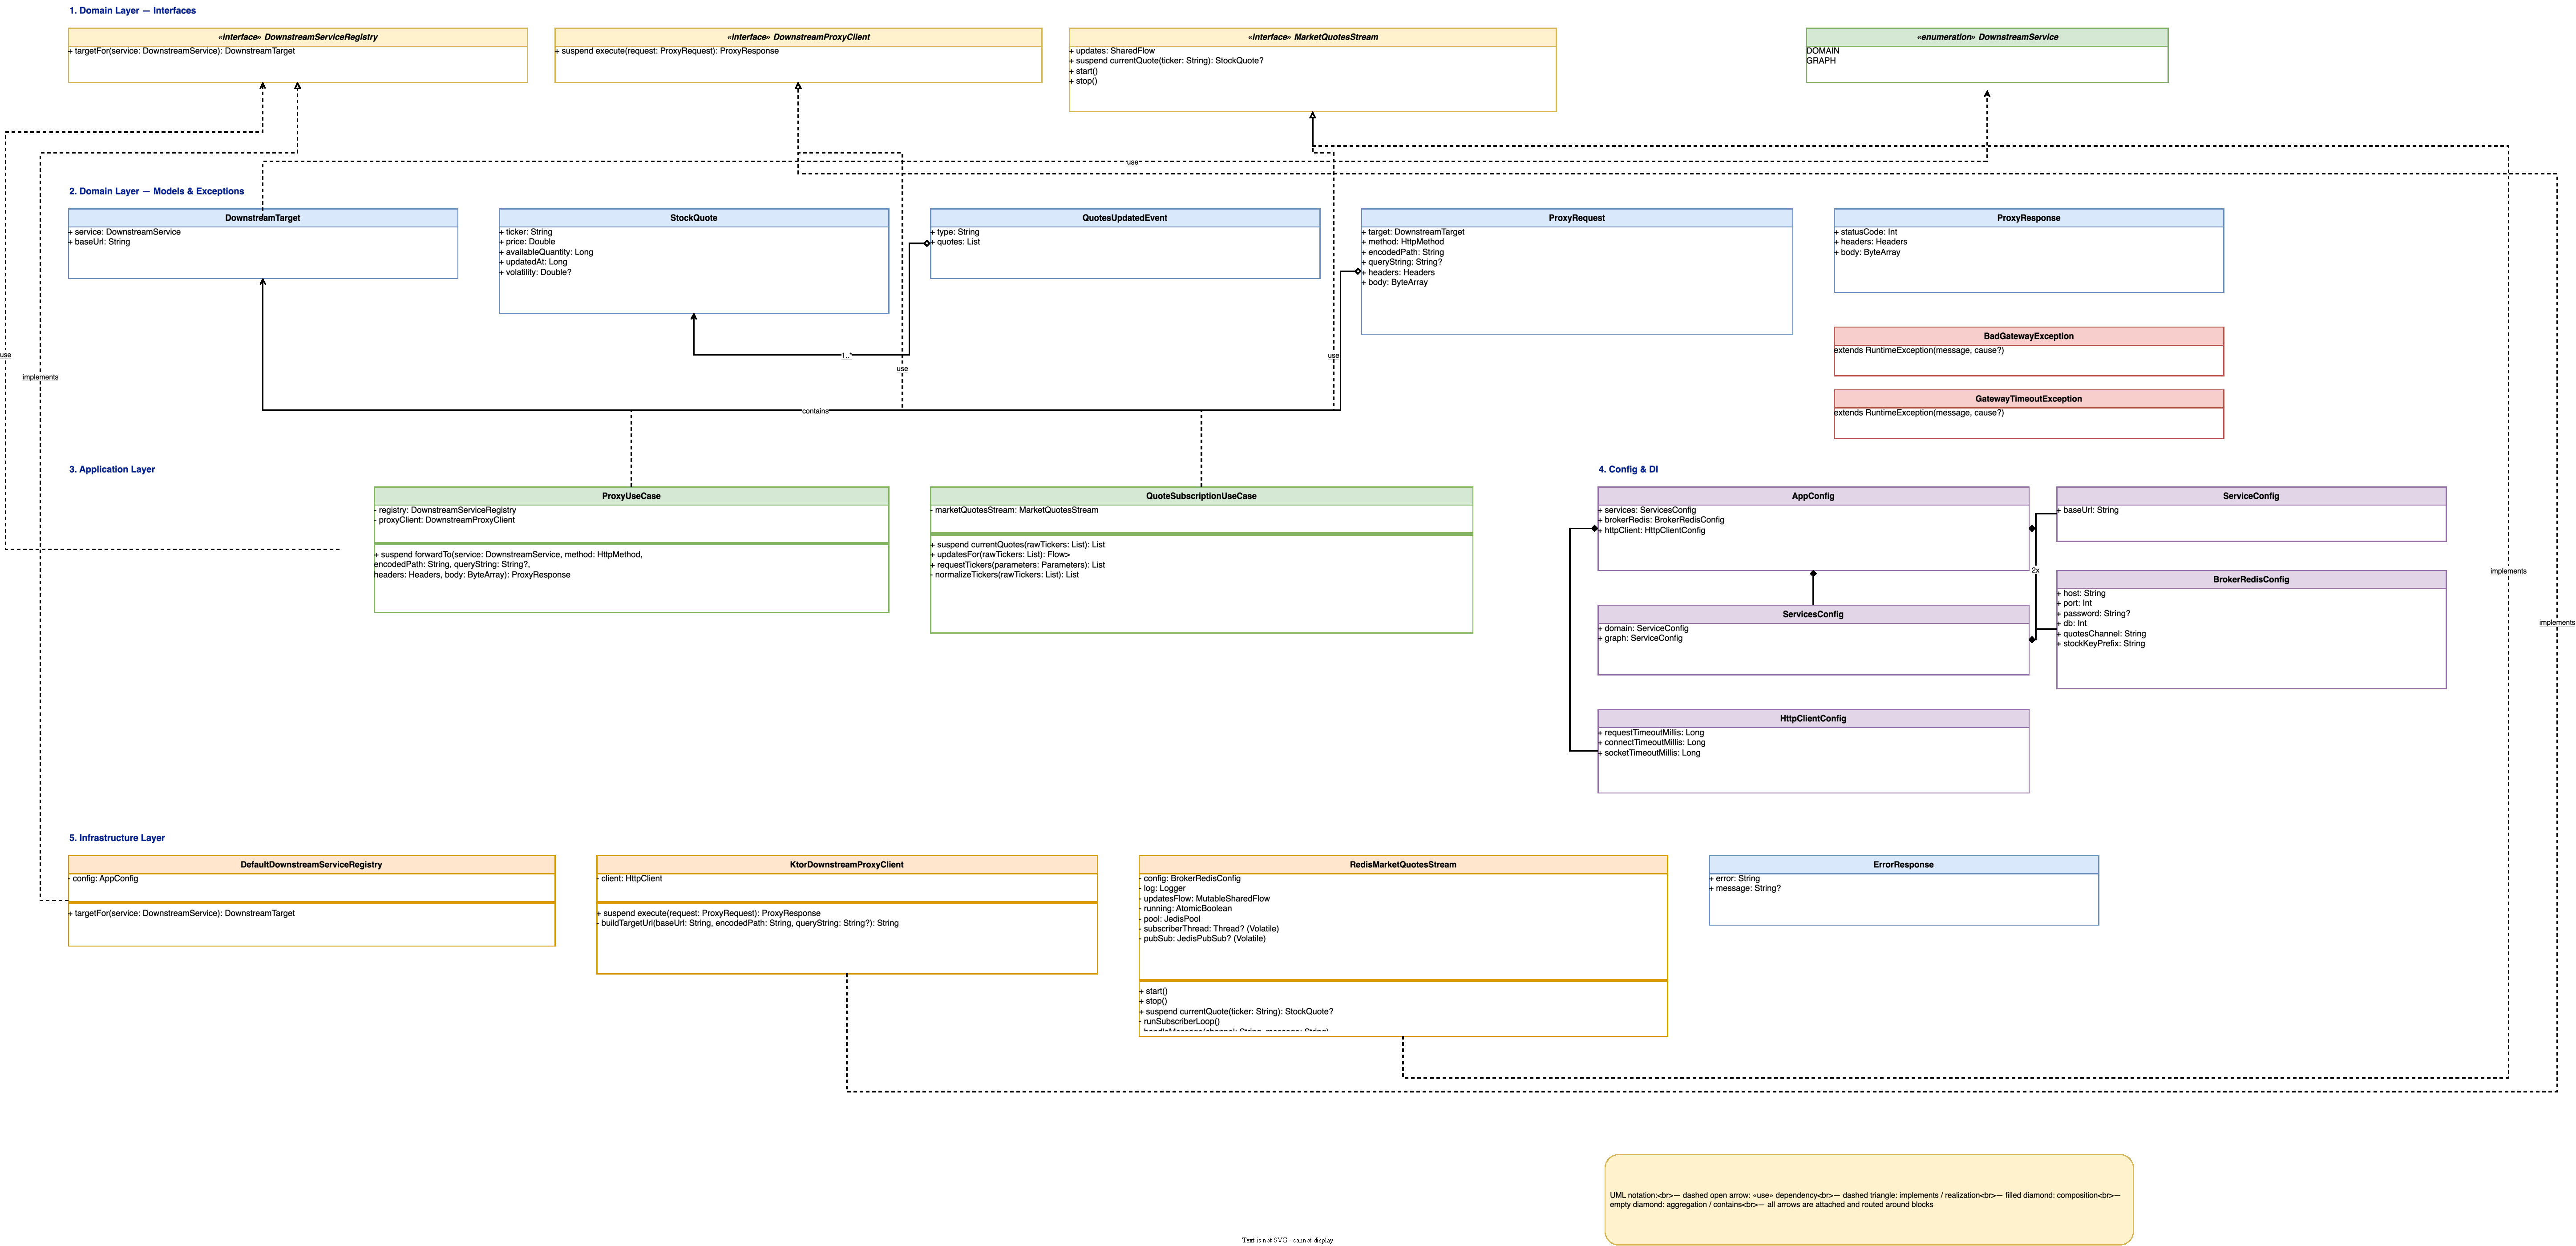
\includegraphics[width=\textwidth]{images/gateway.pdf}
    \caption{Архитектура Gateway-сервиса}
\end{figure}

\newpage
\section{Domain Service}

\begin{figure}[h]
    \centering
    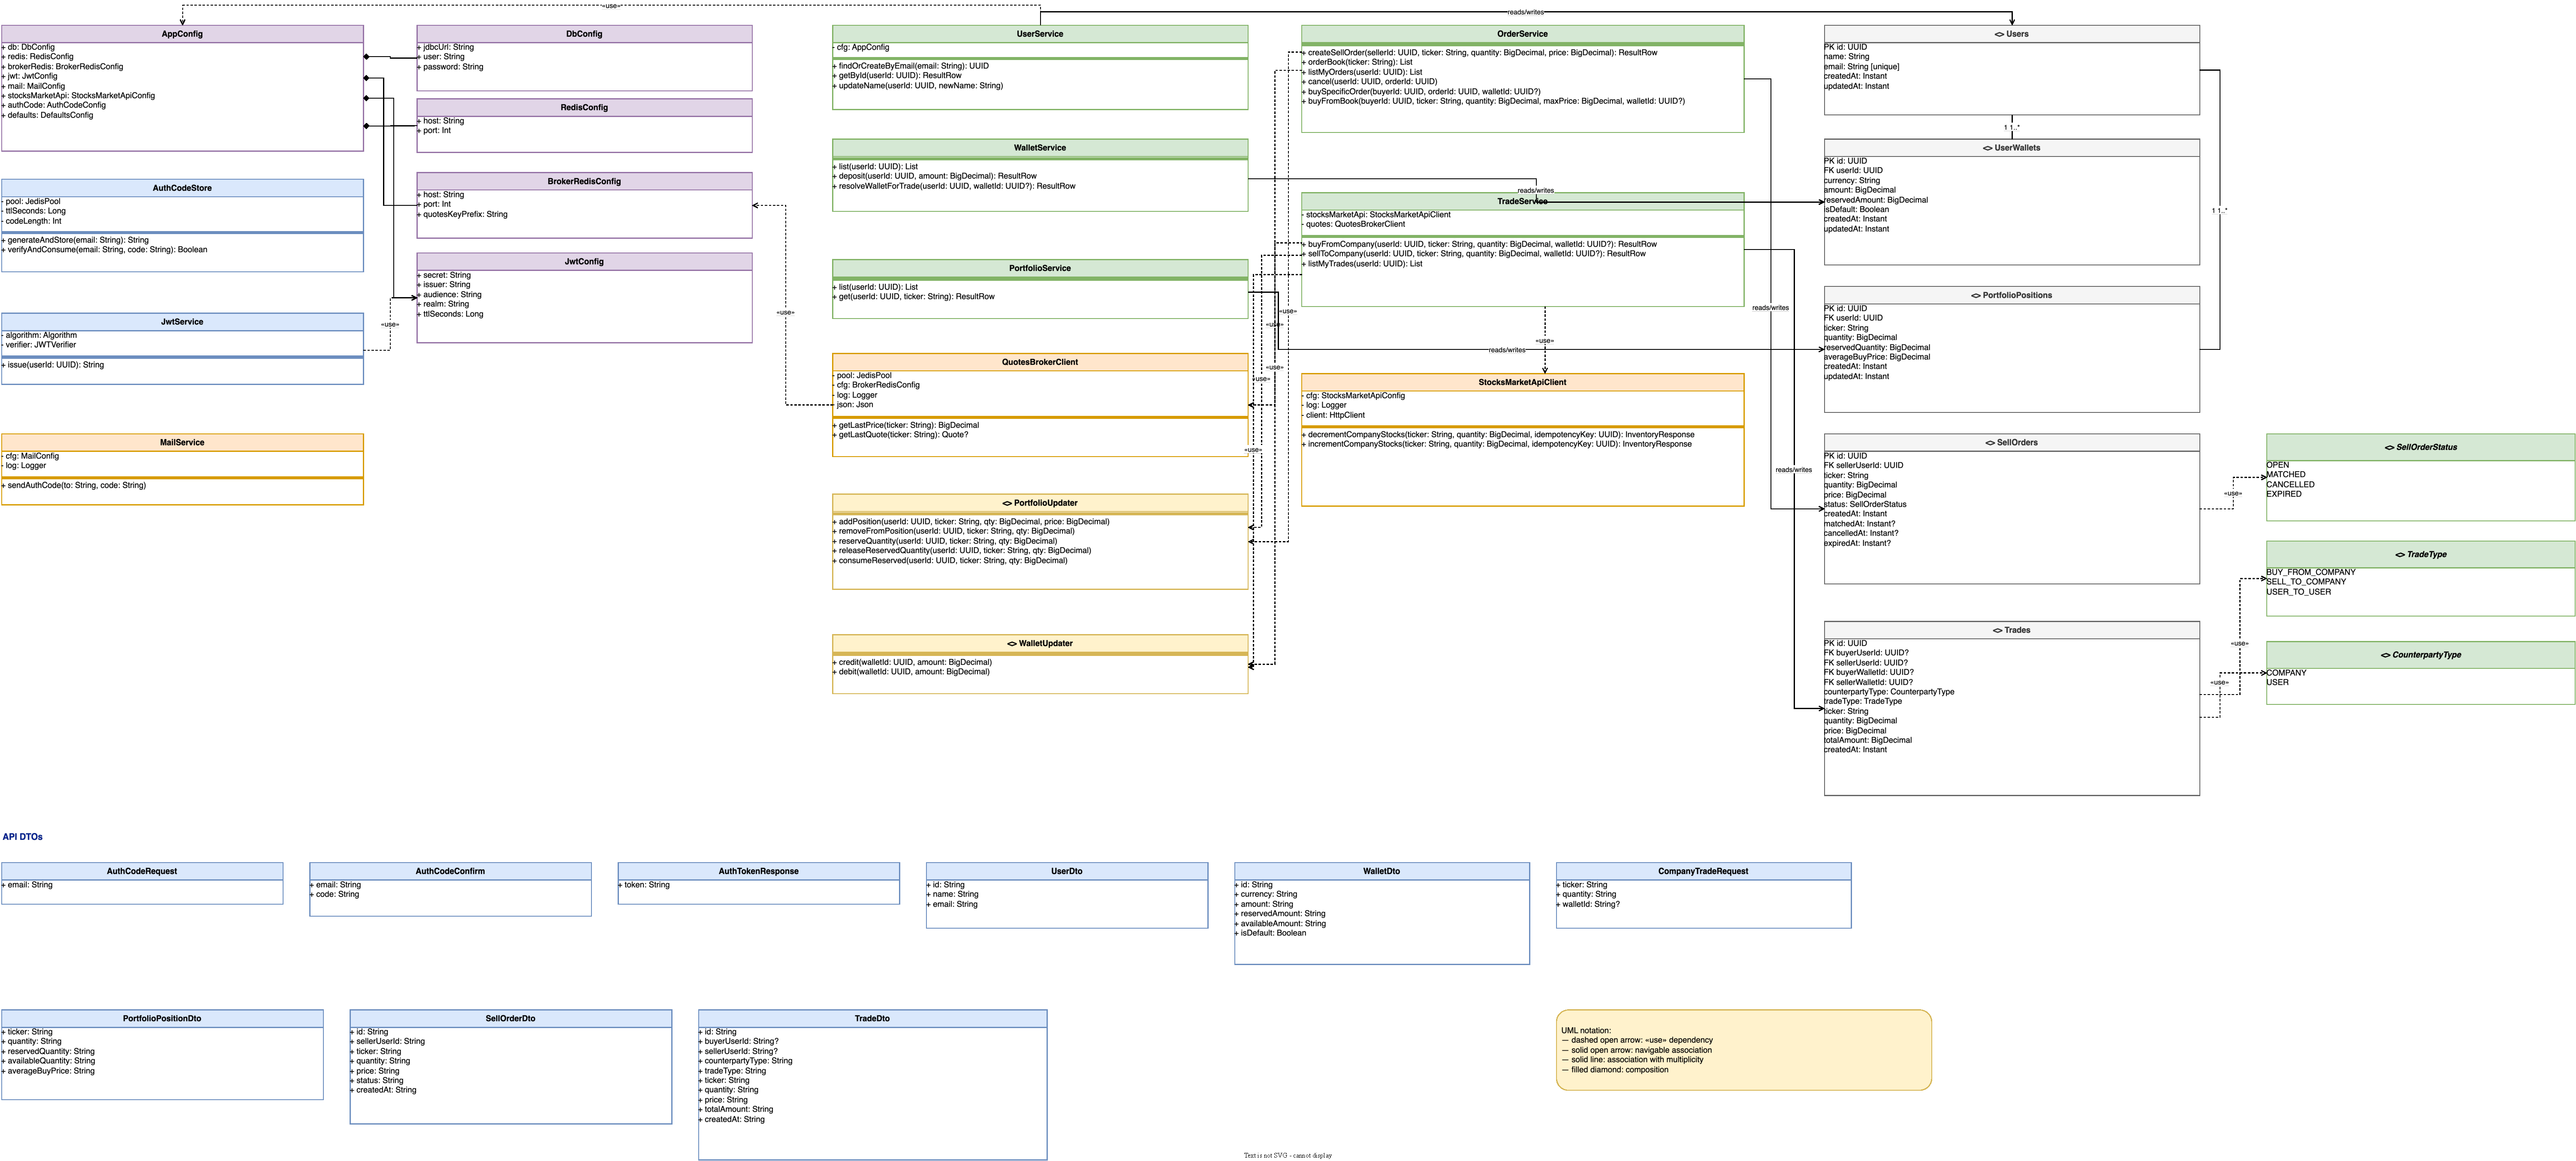
\includegraphics[width=\textwidth]{images/domain-service.pdf}
    \caption{Архитектура Domain Service}
\end{figure}

\newpage
\section{Market Service}

\begin{figure}[h]
    \centering
    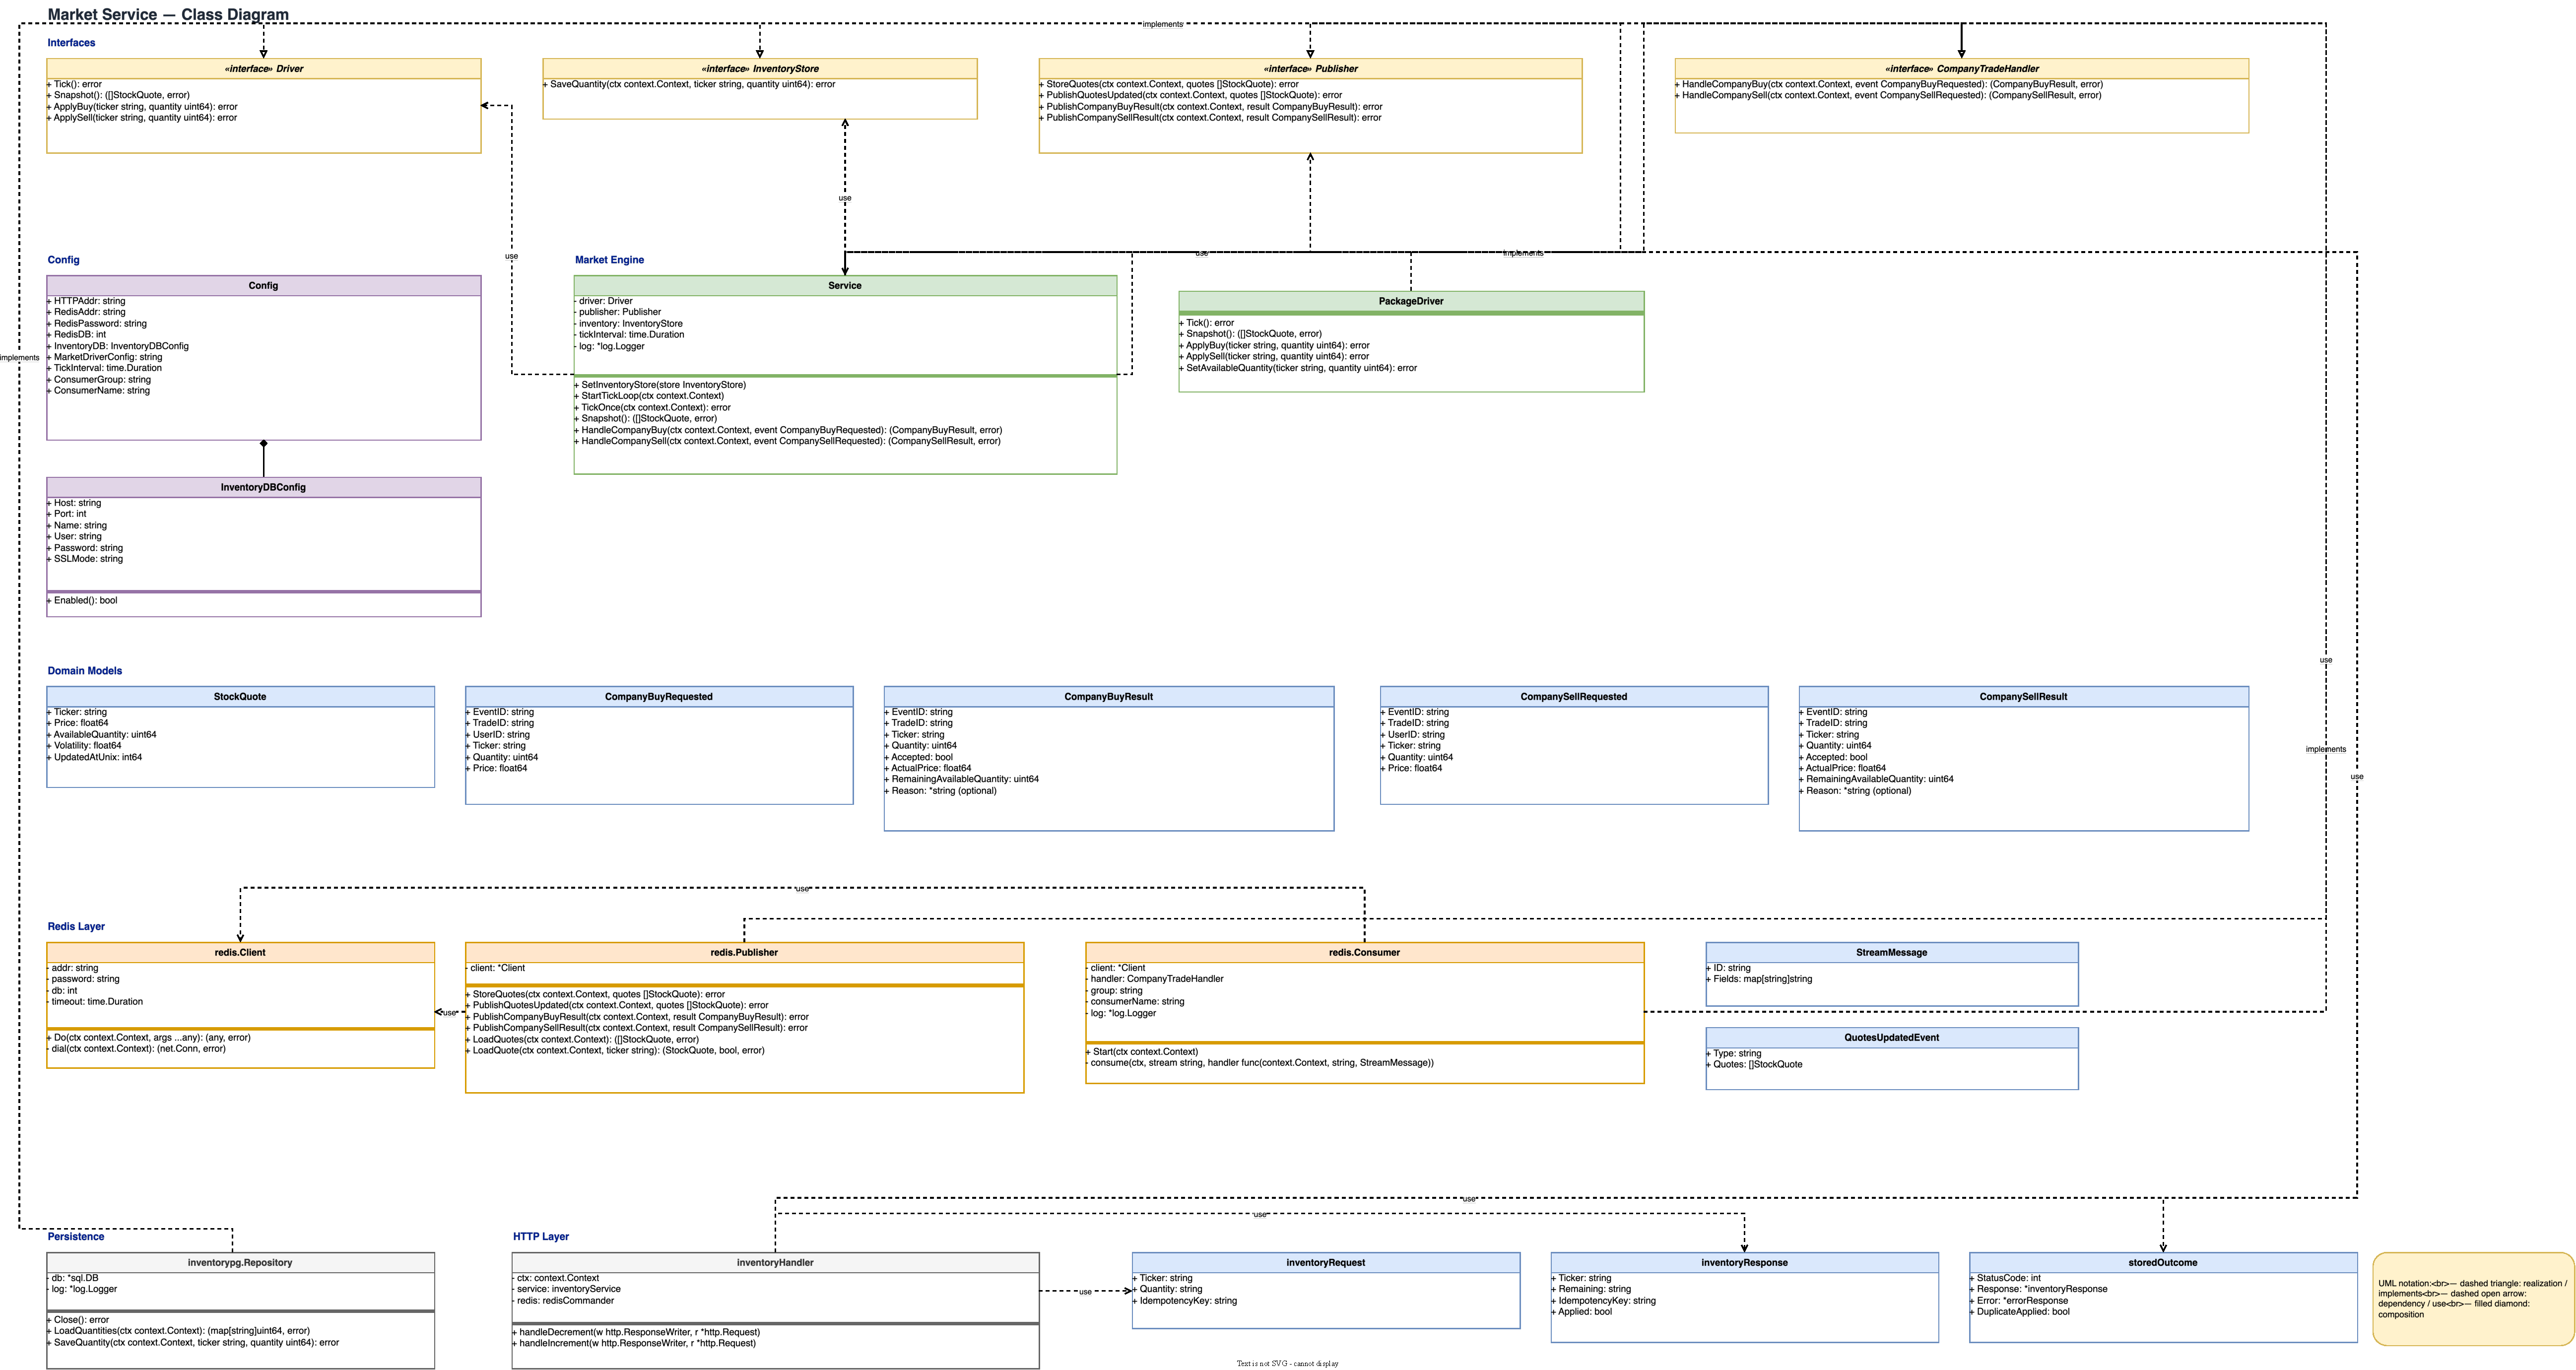
\includegraphics[width=\textwidth]{images/market-service.pdf}
    \caption{Архитектура Market Service (симуляция рынка)}
\end{figure}

\newpage
\section{Graph Service}

\begin{figure}[h]
    \centering
    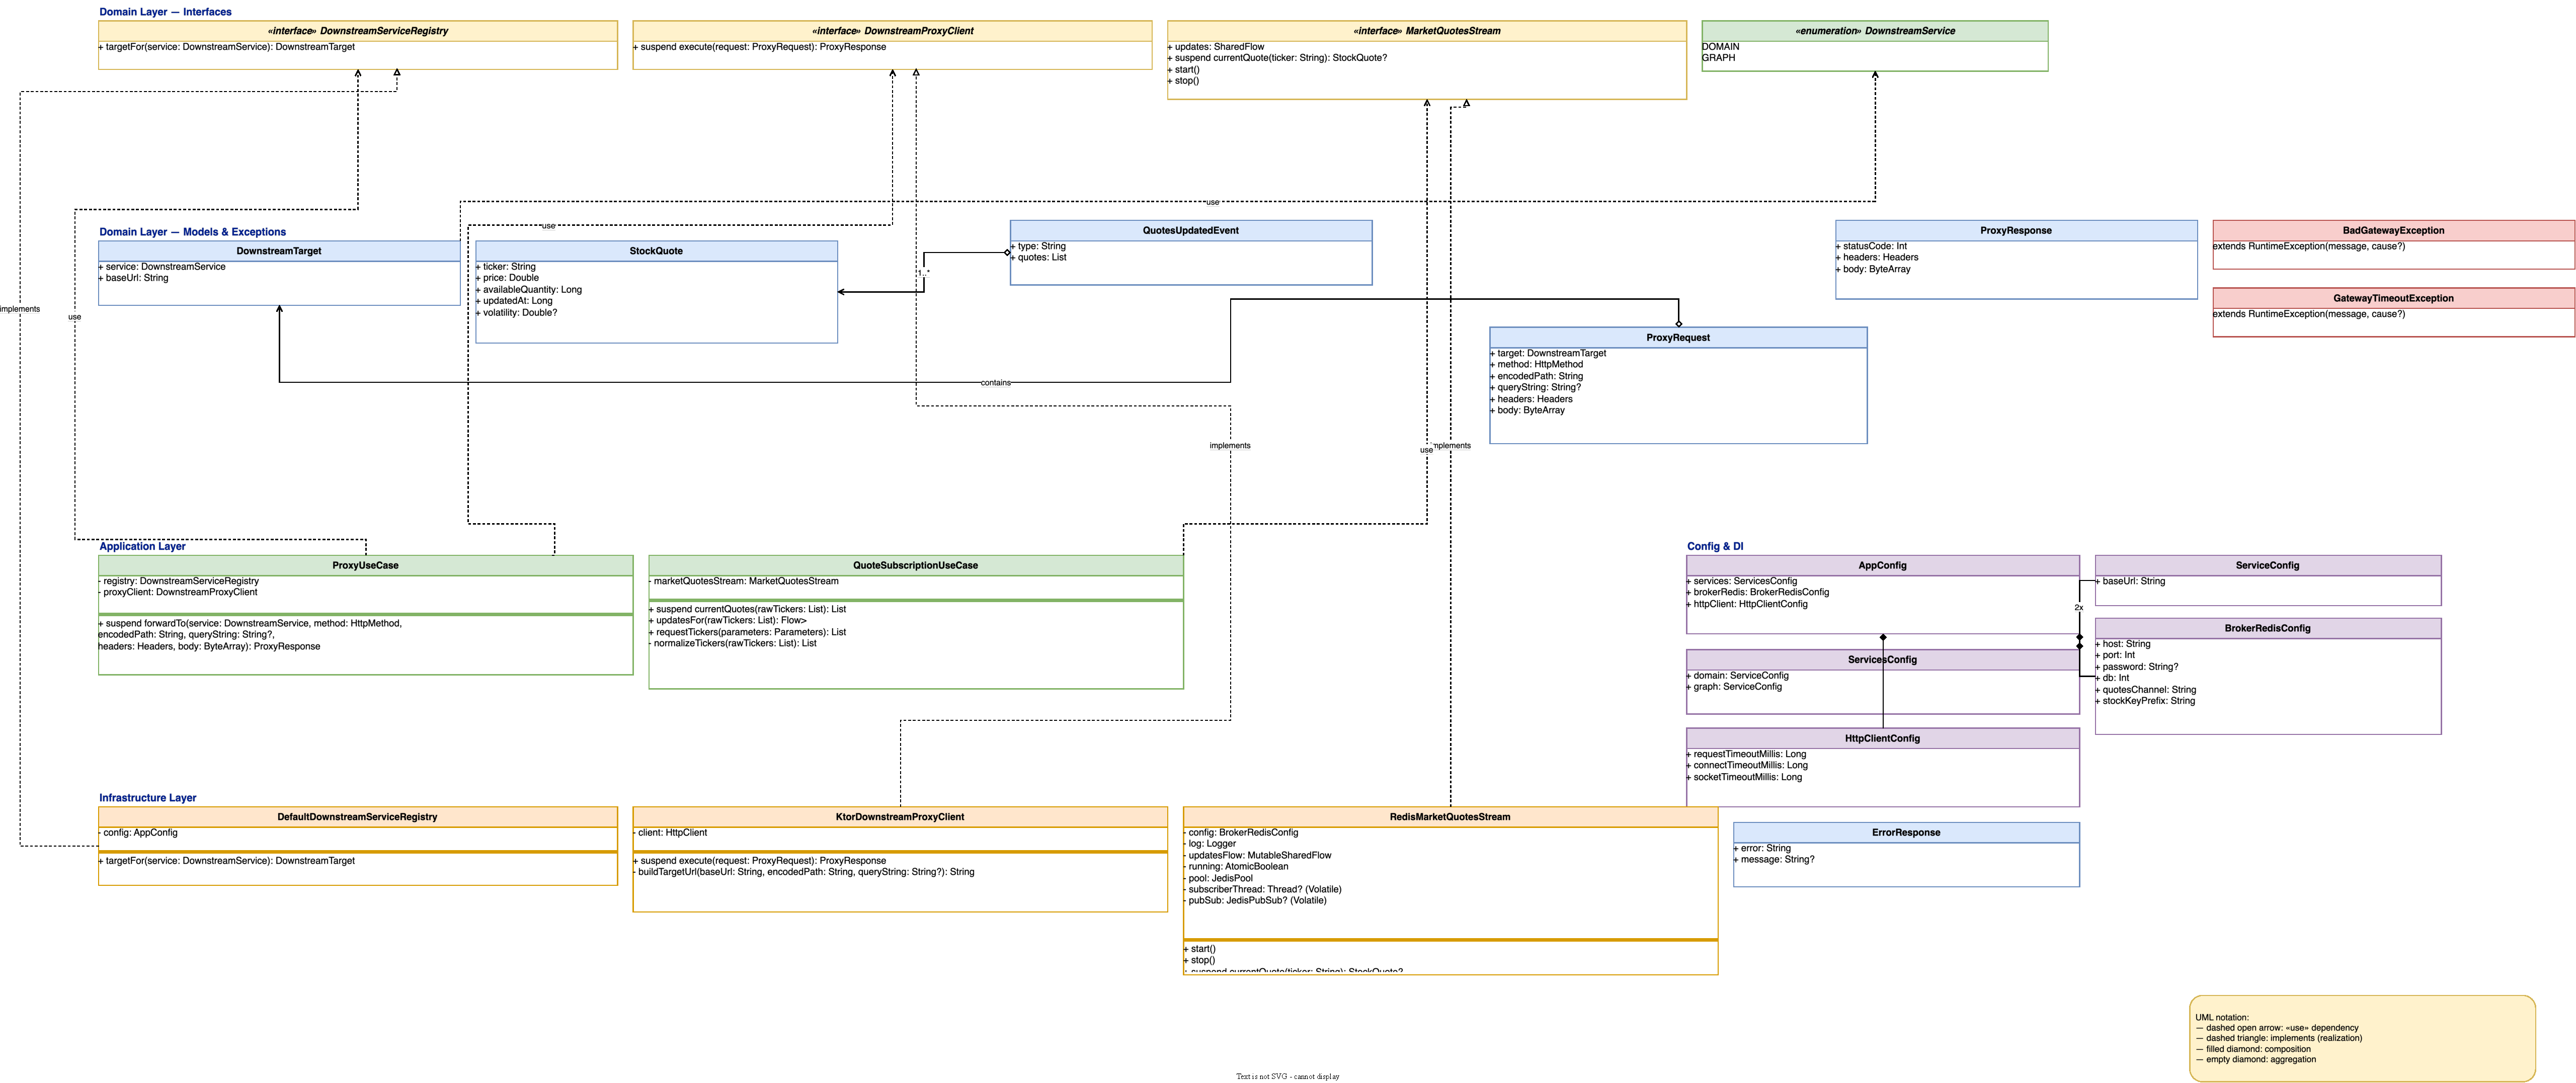
\includegraphics[width=\textwidth]{images/graph-service.pdf}
    \caption{Архитектура Graph Service (история котировок и графики)}
\end{figure}

\end{document}
